\begin{name}
	{ÔN TẬP KIỂM TRA CUỐI HỌC KÌ 1}
	{TOÁN 10}
	{LỚP TOÁN THẦY PHÁT}
	{\thoigian}
\end{name}

\caulc
\Opensolutionfile{ans}[ans/0-HK1-CD-5-CauGiay-HaNoi-2324-Phan-I]

%Câu 1
\begin{ex}%[0-HK1-CD-5-CauGiay-HaNoi-2324]%[VN-MT6, VM020]%[0D3H2-3]
	Trục đối xứng của parabol $(P) \colon y=3x^2+9x+2\,022$ là đường thẳng
	\choice
	{$x= \dfrac{3}{2}$}
	{\True $x= -\dfrac{3}{2}$}
	{$x= -3$}
	{$x= 3$}
	\loigiai{
		Trục đối xứng của parabol $(P)$ là $x=- \dfrac{b}{2a}=- \dfrac{3}{2}$.
	}
\end{ex}
%Câu 2
\begin{ex}%[0-HK1-CD-5-CauGiay-HaNoi-2324]%[VN-MT6, VM020]%[0D3H1-3]
	Cho hàm số $f(x)= \heva{x+ \sqrt{x-2} \quad &\text{khi} \quad x \ge 2\\ 1-3x \quad &\text{khi} \quad x<2}$. Giá trị $f(1)$ bằng
	\choice
	{$2$}
	{$-5$}
	{\True $-2$}
	{$0$}
	\loigiai{
		Khi $x=1<2$ hàm số có dạng $f(x)=1-3x$\\
		Khi đó $f(1)=1-3 \cdot 1=-2$.	
	}
\end{ex}
%Câu 3
\begin{ex}%[0-HK1-CD-5-CauGiay-HaNoi-2324]%[VN-MT6, VM020]%[0D3H2-2]
	Hàm số $y=x^2-4x+11$ đồng biến trên khoảng nào trong các khoảng sau đây?
	\choice
	{$(-\infty;2)$}
	{$(-2;+\infty)$}
	{$(-\infty;+\infty)$}
	{\True $(2;+\infty)$}
	\loigiai{
		Ta có $a=1>0$ nên hàm số đồng biến trên khoảng $\left(- \dfrac{b}{2a};+\infty\right)$.\\
		Tức là hàm só đồng biến trên khoảng $(2;+\infty)$.
	}
\end{ex}
%Câu 4
\begin{ex}%[0-HK1-CD-5-CauGiay-HaNoi-2324]%[VN-MT6, VM020]%[0H5N1-2]
	Cho hình bình hành $ABCD$. Vectơ nào sau đây cùng phương với $\overrightarrow{AB}$?
	\choice
	{\True $\overrightarrow{BA}$, $\overrightarrow{CD}$, $\overrightarrow{DC}$}
	{$\overrightarrow{BA}$, $\overrightarrow{CD}$, $\overrightarrow{CB}$}
	{$\overrightarrow{BC}$, $\overrightarrow{CD}$, $\overrightarrow{DA}$}
	{$\overrightarrow{AD}$, $\overrightarrow{CD}$, $\overrightarrow{DC}$}
	\loigiai{
		\begin{center}
			\begin{tikzpicture}[scale=0.9,font=\footnotesize, line join=round, line cap=round, >=stealth]
				\def\d{4}
				\def\r{3}
				\path (0:0) coordinate (B)
				++(0:\d) coordinate (C)
				++(50:\r) coordinate (D)
				($(B)+(D)-(C)$) coordinate (A);
				\draw (A)--(B)--(C)--(D)--cycle;
				\foreach \x/ \goc in {A/180,B/180,C/0,D/0} 
				\fill (\x) circle (1pt)	
				($(\x)+(\goc:3mm)$) node {$\x$};
			\end{tikzpicture}
		\end{center}
		Các vectơ cùng phương với vectơ $\overrightarrow{AB}$ là $\overrightarrow{BA}$, $\overrightarrow{CD}$, $\overrightarrow{DC}$.
	}
\end{ex}
%Câu 5
\begin{ex}%[0-HK1-CD-5-CauGiay-HaNoi-2324]%[VN-MT6, VM020]%[0H5H3-1]
	Biết $\overrightarrow{AB}=\overrightarrow{a}$. Gọi $C$ là điểm thỏa mãn $\overrightarrow{CA}=\overrightarrow{AB}$. Hãy chọn khẳng định đúng.
	\choice
	{$\overrightarrow{CA}=2 \overrightarrow{a}$}
	{\True $\overrightarrow{CB}=2 \overrightarrow{a}$}
	{$\overrightarrow{AC}=\overrightarrow{0}$}
	{$\overrightarrow{BC}=2 \overrightarrow{a}$}
	\loigiai{
		$C$ là điểm thỏa mãn $\overrightarrow{CA}=\overrightarrow{AB}$ khi đó $A$ là trung điểm của đoạn thẳng $CB$.\\
		Vậy $\overrightarrow{CB}=2 \overrightarrow{AB}=2 \overrightarrow{a}$.
	}
\end{ex}
%Câu 6
\begin{ex}%[0-HK1-CD-5-CauGiay-HaNoi-2324]%[VN-MT6, VM020]%[0D7H2-1]
	Tập hợp tất cả các giá trị của $x$ để đa thức $f(x)=x^2-6x+8$ không dương là
	\choice
	{$[2;3]$}
	{\True $[2;4]$}
	{$[1;4]$}
	{$(-\infty;2] \cup [4;+\infty)$}
	\loigiai{
		Đa thức $f(x)=x^2-6x+8$ không dương, tức là
		\[x^2-6x+8 \le 0 \Leftrightarrow 2 \le x \le 4.\]
	}
\end{ex}
%Câu 7
\begin{ex}%[0-HK1-CD-5-CauGiay-HaNoi-2324]%[VN-MT6, VM020]%[0D2H2-2]
	Điểm $O(0;0)$ \textbf{không} thuộc miền nghiệm của hệ bất phương trình nào sau đây?
	\choice
	{$\heva{&x+3y \ge 0\\ &2x+y-4<0}$}
	{$\heva{&x+3y-6 < 0\\ &2x+y+4 \ge 0}$}
	{\True $\heva{&x+3y < 0\\ &2x+y+4>0}$}
	{$\heva{&x+3y-6 < 0\\ &2x+y+4>0}$}
	\loigiai{
		Thay tọa độ điểm $O(0;0)$ vào các đáp án ta thấy đáp án $\heva{&x+3y < 0\\ &2x+y+4>0}$ không thỏa mãn nên điểm $O(0;0)$ không thuộc miền nghiệm của hệ.
	}
\end{ex}
%Câu 8
\begin{ex}%[0-HK1-CD-5-CauGiay-HaNoi-2324]%[VN-MT6, VM020]%[0D7H2-1]
	Tìm tập xác định của hàm số $y= \sqrt{2x^2-5x+2}$.
	\choice
	{$\left[\dfrac{1}{2};2\right]$}
	{$\left(-\infty;\dfrac{1}{2}\right]$}
	{\True $\left(-\infty;\dfrac{1}{2}\right] \cup \left[2;+\infty\right)$}
	{$\left[2;+\infty\right)$}
	\loigiai{
		Hàm số xác định khi và chỉ khi $2x^2-5x+2 \ge 0$
		$\Leftrightarrow \hoac{&x \le \dfrac{1}{2}\\ &x \ge 2.}$\\
		Vậy tập xác định của hàm số là $\mathscr{D}=\left(-\infty;\dfrac{1}{2}\right] \cup \left[2;+\infty\right)$.
	}
\end{ex}
%Câu 9
\begin{ex}%[0-HK1-CD-5-CauGiay-HaNoi-2324]%[VN-MT6, VM020]%[0D3H2-3]
	\immini[thm]{Cho đồ thị hàm số $y=a x^2+b x+c$ có đồ thị như hình vẽ. Mệnh đề nào sau đây đúng?
		\choice[2]
		{$a>0$, $b=0$, $c>0$}
		{$a<0$, $b>0$, $c>0$}
		{\True $a>0$, $b<0$, $c>0$}
		{$a>0$, $b>0$, $c>0$}}
	{	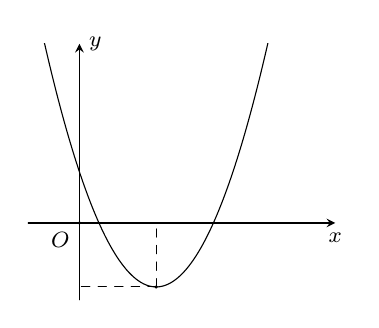
\begin{tikzpicture}[scale=.65,font=\footnotesize, line join=round, line cap=round, >=stealth]
			\def\a{1} % Hệ số a phải khác 0
			\def\b{-3}
			\def\c{1}
			\draw[->] (-1,0) -- (5,0) node[below] {$x$};
			\draw[->] (0,-1.5) -- (0,3.5) node[right] {$y$};
			\draw (0,0)node[below left]{$O$};
			\pgfmathsetmacro\xdinh{-(\b)/2*(\a)}
			\pgfmathsetmacro\ydinh{(4*(\a)*(\c)-(\b)^2)/(4*(\a))}
			\fill[dashed] (\xdinh,\ydinh)circle(1pt) edge (\xdinh,0) edge (0,\ydinh);
			\fill (0,0) circle (1pt);
			\clip (-1,-1.5)rectangle(5,3.5);
			\draw[samples=150,smooth,domain=-1:5] plot(\x,{\a*(\x)^2+(\b)*\x+(\c)});
		\end{tikzpicture}
	}	
	\loigiai{
		\begin{itemize}
			\item 	Parabol đã cho có bề lõm hướng lên trên nên hàm số đã cho có hệ số $a>0$.
			\item Parabol cắt trục tung tại điểm có tung độ dương nên $c>0$.
			\item Parabol có đỉnh nằm ở góc phần tư thứ $IV$ nên hoành độ đỉnh dương. Tức là $-\dfrac{b}{2a}>0$. Vì $a>0$ nên từ đây ta có $b<0$.
		\end{itemize}
	}
\end{ex}

%Câu 10
\begin{ex}%[0-HK1-CD-5-CauGiay-HaNoi-2324]%[VN-MT6, VM020]%[0D3N2-1]
	Trong các hàm số sau, hàm số nào là hàm số bậc hai?
	\choice
	{\True $y=2 x(3-x)$}
	{$y=2 x-3$}
	{$y=\dfrac{2 x^2+6 x-1}{x^2+x+1}$}
	{$y=x\left(2 x^2-3\right)$}
	\loigiai{ Ta có $y=2 x(3-x)=-2x^2+6x$. Đây là hàm số bậc hai với các hệ số $a=-2$, $b=6$, $c=0$.		
	}
\end{ex}

%Câu 11
\begin{ex}%[0-HK1-CD-5-CauGiay-HaNoi-2324]%[VN-MT6, VM020]%[0H5H3-4]
	Biết rằng hai vectơ $\overrightarrow{a}$ và $\overrightarrow{b}$ không cùng phương nhưng hai vectơ $\overrightarrow{u}=3 \overrightarrow{a}-2 \overrightarrow{b}$ và $\overrightarrow{v}=(x+1) \overrightarrow{a}+4 \overrightarrow{b}$ cùng phương. Khi đó giá trị của $x$ là
	\choice
	{\True $-7$}
	{$6$}
	{$5$}
	{$7$}
	\loigiai{Vì hai vectơ $\overrightarrow{a}$ và $\overrightarrow{b}$ không cùng phương nên $\overrightarrow{u}=3 \overrightarrow{a}-2 \overrightarrow{b} \ne \overrightarrow{0}$.\\
		Hai vectơ $\overrightarrow{u}$ và $\overrightarrow{v}$ cùng phương khi và chỉ khi tồn tại số thực $k$ sao cho $\overrightarrow{v}=k \overrightarrow{ u}$, tức là
		\[(x+1) \overrightarrow{a}+4 \overrightarrow{b}=k\left(3 \overrightarrow{a}-2 \overrightarrow{b}\right)\Leftrightarrow (x-3k+1) \overrightarrow{a}+(4+2k)\overrightarrow{b}=\overrightarrow{0}\Leftrightarrow \heva{&x-3k+1=0\\&4+2k=0}\Leftrightarrow\heva{&x=-7\\&k=-2.}\]}
\end{ex}

%Câu 12
\begin{ex}%[0-HK1-CD-5-CauGiay-HaNoi-2324]%[VN-MT6, VM020]%[0H5H3-1]
	Cho tam giác $ABC$ vuông cân tại $A$ có $AB=a$. Tính $\left|\overrightarrow{AB}+\overrightarrow{AC}\right|$.
	\choice
	{\True $\left|\overrightarrow{AB}+\overrightarrow{AC}\right|=a \sqrt{2}$}
	{$\left|\overrightarrow{AB}+\overrightarrow{AC}\right|=a$}
	{$\left|\overrightarrow{AB}+\overrightarrow{AC}\right|=\dfrac{a \sqrt{2}}{2}$}
	{$\left|\overrightarrow{AB}+\overrightarrow{AC}\right|=2a$}
	\loigiai{
		\begin{center}
			\begin{tikzpicture}[scale=0.9,font=\footnotesize, line join=round, line cap=round, >=stealth]
				\def\r{3}
				\path 	(180:\r) coordinate (B)
				(0:\r) coordinate (C)	
				($(B)!0.5!(C)$) coordinate (I)
				node at ($(B)!0.5!(C)$) [below] {$I$}	
				($(I)+(90:\r)$) coordinate (A);
				\draw (A)--(B)--(C)--cycle (A)--(I)
				pic[draw,angle radius=2mm]{right angle=B--A--C};
				\foreach \x/ \goc in {A/135,B/-135,C/-90} 
				\fill (\x) circle (1pt)
				($(\x)+(\goc:3mm)$) node {$\x$};	
				
			\end{tikzpicture}
		\end{center}
		Gọi $I$ là trung điểm của cạnh $BC$, khi đó ta có $\overrightarrow{AB}+\overrightarrow{AC}=2\overrightarrow{AI}$, suy ra
		\[\left|\overrightarrow{AB}+\overrightarrow{AC} \right| =2 \left| \overrightarrow{AI} \right| = 2AI=BC =\sqrt{AB^2+AC^2}=a \sqrt{2}.\]
	}
\end{ex}
\Closesolutionfile{ans}

%================================PHẦN II
\cauds
\Opensolutionfile{ans}[ans/0-HK1-CD-5-CauGiay-HaNoi-2324-Phan-II]

%Câu 1
\begin{ex}%[0-HK1-CD-5-CauGiay-HaNoi-2324]%[VN-MT6, VM020]%[0H5H3-5]
	Cho tam giác $ABC$ có trọng tâm $G$, gọi $M$ là trung điểm $BC$.
	\choiceTF
	{\True $\overrightarrow{A G}=\dfrac{1}{3}\overrightarrow{AB}+\dfrac{1}{3}\overrightarrow{AC}$}
	{$\overrightarrow{GM}=\overrightarrow{GB}+\overrightarrow{GC}$}
	{\True $\overrightarrow{AG}=\overrightarrow{GB}+\overrightarrow{GC}$}
	{$\overrightarrow{GA}=2\overrightarrow{GM}$}
	\loigiai{
		\begin{center}
			\begin{tikzpicture}[scale=0.9,font=\footnotesize,line join=round,line cap=round,>=stealth]
				\path 
				(0,0)coordinate(O)
				(-3,0)coordinate(B) 
				(1,3)coordinate(A) 
				(3,0)coordinate(C);
				\coordinate (M) at ($(B)!1/2!(C)$);
				\coordinate (G) at ($(A)!2/3!(M)$);
				\foreach \p/\g in {A/90,B/180,C/0,M/-90,G/0}
				\draw[fill=black] (\p) circle (1pt) node[shift=(\g:3mm)] {$\p$};				
				\draw (A)--(B)--(C)--(A)--(M);	
			\end{tikzpicture}
		\end{center}
		\begin{itemchoice}
			\itemch \textbf{Đúng.}\\ 	Vì $M$ là trung điểm của $BC$ nên $\overrightarrow{A M}=\dfrac{1}{2}\overrightarrow{A B}+\dfrac{1}{2}\overrightarrow{A C}$.\\
			Vì $G$ là trọng tâm tam giác $ABC$ nên 
			\[\overrightarrow{A G}=\dfrac{2}{3}\overrightarrow{AM}=\dfrac{2}{3}\left(\dfrac{1}{2}\overrightarrow{A B}+\dfrac{1}{2}\overrightarrow{A C}\right)=\dfrac{1}{3}\overrightarrow{A B}+\dfrac{1}{3}\overrightarrow{A C}.\] 
			\itemch \textbf{Sai.}\\ Vì $M$ là trung điểm của $BC$ nên $\overrightarrow{GB}+\overrightarrow{GC}=2\overrightarrow{GM}$.
			\itemch \textbf{Đúng.}\\ Vì $G$ là trọng tâm tam giác $ABC$ nên $\overrightarrow{GA}+\overrightarrow{GB}+\overrightarrow{GC}=\overrightarrow{0}$.\\
			Suy ra $\overrightarrow{GB}+\overrightarrow{GC}=-\overrightarrow{GA}=\overrightarrow{AG}$.
			\itemch \textbf{Sai.}\\ Ta có $\overrightarrow{GA}=-2\overrightarrow{GM}$.
		\end{itemchoice}		
	}
\end{ex}
%Câu 2
\begin{ex}%[0-HK1-CD-5-CauGiay-HaNoi-2324]%[VN-MT6, VM020]%[0H5H3-6]
	Cho hình thoi $ABCD$ có cạnh bằng $a$ và $\widehat{A}=60^{\circ}$. Gọi $O$ là tâm hình thoi.
	\choiceTF
	{$\left|\overrightarrow{BA}+\overrightarrow{BC}\right|=2a$}
	{\True $\left|\overrightarrow{AB}+\overrightarrow{OD}\right|=\dfrac{a\sqrt{3}}{2}$}
	{\True $\left|\overrightarrow{OA}+\overrightarrow{OB}\right|=a$}
	{\True $\left|\overrightarrow{DA}+\overrightarrow{DC}\right|=a$}
	\loigiai{
		\begin{center}
			\begin{tikzpicture}[scale=1,font=\footnotesize,line join=round,line cap=round,>=stealth]
				\def\a{3.2}
				\path 
				(0,0) coordinate(A)
				(30:\a) coordinate(B)
				(-30:\a) coordinate(D)
				($(B)!1/2!(D)$) coordinate(O)
				($2*(O)-(A)$) coordinate(C)
				($(A)!0.5!(B)$)coordinate (M);
				\foreach \p/\g in {A/180,B/90,C/0,O/-45,D/-90,M/135}
				\fill (\p) circle (1pt) node[shift=(\g:3mm)] {$\p$};
				\draw (A)--(B)--(C)--(D)--(A) (A)--(C) (B)--(D) (O)--(M);
			\end{tikzpicture}
		\end{center}
		Tam giác $ABD$ cân tại $A$ và $\widehat{A}=60^{\circ}$ nên đây là tam giác đều. \\
		Vì tam giác $ABD$ đều, cạnh bằng $a$ nên $BO=\dfrac{1}{2}BD=\dfrac{a}{2}$.	
		\begin{itemchoice}
			\itemch \textbf{Sai.}\\ Ta có $\overrightarrow{B A}+\overrightarrow{B C}=2\overrightarrow{BO}$.\\
			Vậy $\left|\overrightarrow{B A}+\overrightarrow{B C}\right|=\left|2\overrightarrow{BO}\right|=2BO=a$.
			\itemch \textbf{Đúng.}\\ Ta có $\left|\overrightarrow{AB}+\overrightarrow{OD}\right|=\left|\overrightarrow{AB}+\overrightarrow{BO}\right|=\left|\overrightarrow{AO}\right|=\dfrac{a\sqrt{3}}{2}$.
			\itemch \textbf{Đúng.}\\ Gọi $M$ là trung điểm của $AB$. Ta có $\overrightarrow{OA}+\overrightarrow{OB}=2\overrightarrow{OM}$.\\ Suy ra $\left|\overrightarrow{OA}+\overrightarrow{OB}\right|=\left|2\overrightarrow{OM}\right|=2\cdot OM=AB=a$.
			\itemch \textbf{Đúng.}\\ Ta có $\left|\overrightarrow{DA}+\overrightarrow{DC}\right|=\left|\overrightarrow{DB}\right|=DB=a$.
		\end{itemchoice}	
	}
\end{ex}
%Câu 3
\begin{ex}%[0-HK1-CD-5-CauGiay-HaNoi-2324]%[VN-MT6, VM020]%[0D3H2-1]
	Biết parabol $(P)\colon y=2x^2+bx+c$ đi qua điểm $M(0;4)$ và có trục đối xứng là đường thẳng $x=1$.
	\choiceTF
	{\True $b+c=0$}
	{$b>0$, $c>0$}
	{Parabol $(P)$ cắt trục hoành tại hai điểm phân biệt}
	{\True Parabol $(P)$ có đỉnh là $I(1;2)$}
	\loigiai{
		\begin{itemize}
			\item Parabol $(P)$ đi qua điểm $M(0 ; 4)$ nên $4=2\cdot 0^2+b\cdot 0+c \Leftrightarrow c=4$.
			\item Parabol có trục đối xứng là đường thẳng $x=1$ nên $-\dfrac{b}{2a}=1\Leftrightarrow b=-4$.
		\end{itemize}
		\begin{itemchoice}
			\itemch \textbf{Đúng.}\\ $b+c=-4+4=0$.
			\itemch \textbf{Sai.}\\ $b=-4<0$, $c=4>0$
			\itemch \textbf{Sai.}\\ Parabol $(P)\colon y=2x^2-4x+4$.\\
			Phương trình hoành độ giao điểm của $(P)$ và trục hoành là $2x^2-4x+4=0$. Phương trình vô nghiệm nên $(P)$ không cắt trục hoành.
			\itemch \textbf{Đúng.}\\ Parabol $(P)\colon y=2x^2-4x+4$ có $a=2$, $b=-4$, $c=4$.\\
			Ta có $-\dfrac{b}{2a}=1$, $-\dfrac{\Delta}{4a}=2$.\\
			Vậy parabol $(P)$ có đỉnh là $I(1;2)$.
		\end{itemchoice}	
	}
\end{ex}
%Câu 4
\begin{ex}%[0-HK1-CD-5-CauGiay-HaNoi-2324]%[VN-MT6, VM020]%[0D3H1-7]
	Bảng giá cước của một hãng taxi được cho như sau
	\begin{center}
		\renewcommand\arraystretch{1.2}
		\begin{tabular}{|c|c|}
			\hline Giá mở cửa & Giá km tiếp theo \\
			\hline $11\,000 \text{\,đ}/ 0{,}7 \mathrm{\,km}$ & $15\,800 \text{\,đ}/ 1{,}0 \mathrm{\,km}$ \\
			\hline
		\end{tabular}
	\end{center}
	(\textit{Giá mở cửa: Khi lên taxi mà quãng đường di chuyển không quá $0{,}7$ km thì hãng taxi vẫn tính $11\,000$ đồng}). Gọi $y$ (đồng) là số tiền phải trả sau khi đi $x$ (km).
	\choiceTF
	{Số tiền phải trả khi đi $10$ \,km là $157\,850$ \,đồng}
	{\True Số tiền phải trả khi đi $50$ \,km là $789\,940$ \,đồng}
	{\True Với số tiền $1\,000\,000$ đồng, người đó không thể đi taxi với quãng đường vượt quá $64$\,km}
	{\True Hàm số của $y$ theo $x$ là $y=\heva{& 11\,000 &\text{khi}\; x \leq 0{,}7 \\& 15\,800 x-60 & \text{khi}\;x>0{,}7}$}
	\loigiai{
		Ta có $y=\heva{&11\,000 & \text{khi}\;x \leq 0{,}7 \\& 11\,000+(x-0{,}7)15\,800 & \text{khi}\;x>0{,}7}\Leftrightarrow y=\heva{& 11\,000 & \text{khi}\; x \leq 0{,}7 \\& 15\,800 x-60 & \text{khi}\;x>0{,}7.}$
		\begin{itemchoice}
			\itemch \textbf{Sai.}\\ Vì $x=10>0{,}7$ nên số tiền phải trả là $y=15\,800\cdot 10-60=157\,940$\,đồng.
			\itemch \textbf{Đúng.}\\ Số tiền phải trả khi đi $50 \mathrm{\,km}$ là $15\,800\cdot 50-60=789\,940$\,đồng.
			\itemch \textbf{Đúng.}\\ Với $y=1\,000\,000$ ta có 
			\[1\,000\,000=15\,800x-60
			\Leftrightarrow x=\dfrac{50\,003}{790}\approx 63{,}3.
			\]
			\itemch \textbf{Đúng.}\\ Ta có $y=\heva{&11\,000 & \text{khi}\;x \leq 0{,}7 \\& 11\,000+(x-0{,}7)15\,800 & \text{khi}\;x>0{,}7}\Leftrightarrow y=\heva{& 11\,000 & \text{khi}\; x \leq 0{,}7 \\& 15\,800 x-60 & \text{khi}\;x>0{,}7.}$
		\end{itemchoice}
	}
\end{ex}

\Closesolutionfile{ans}

%================================PHẦN III
\caukq
\Opensolutionfile{ans}[ans/0-HK1-CD-5-CauGiay-HaNoi-2324-Phan-III]

%Câu 1
\begin{ex}%[0-HK1-CD-5-CauGiay-HaNoi-2324]%[VN-MT6, VM020]%[0D7H2-6]
	Có bao nhiêu giá trị nguyên của tham số $m\in [0;2\,024]$ để hàm số \[y=\sqrt{(m-2)x^2-2(m-3)x+m-1}\] có tập xác định là $\mathbb{R}$?
	\shortans{$2\,022$}
	\loigiai{
		Hàm số $y=\sqrt{(m-2)x^2-2(m-3)x+m-1}$ có tập xác định là $\mathbb{R}$ khi và chỉ khi 
		\[f(x)=(m-2)x^2-2(m-3)x+m-1 \ge 0, \forall x \in \mathbb{R}.\]
		\begin{itemize}
			\item Trường hợp 1: Nếu $m-2=0\Leftrightarrow m=2$.\\
			Khi đó $f(x)=2x+1$, $f(x)\ge 0\Leftrightarrow x\ge -\dfrac{1}{2}$.\\
			Suy ra $m=2$ không thoả mãn.
			\item Trường hợp 2: Nếu $m-2\neq 0\Leftrightarrow m\neq 2$.
			\begin{eqnarray*}
				&&(m-2)x^2-2(m-3)x+m-1 \ge 0, \forall x \in \mathbb{R}\\
				&\Leftrightarrow& \heva{&m-2>0\\ &\Delta' \le 0}\\
				&\Leftrightarrow& \heva{&m>2\\ &(m-3)^2-(m-2)(m-1) \le 0}\\
				&\Leftrightarrow& \heva{&m>2\\ &-3m+7 \le 0}\\
				&\Leftrightarrow& \heva{&m>2\\ &m \ge \dfrac{7}{3}}\\
				&\Leftrightarrow& m \ge \dfrac{7}{3}.
			\end{eqnarray*}	
			Vì $m\in\mathbb{Z}$, $m\in [0;2\,024]$ nên $m\in \{3;4;\ldots;2\,024\}$.\\
			Vậy có $2\,022$ giá trị $m$ thoả mãn.
		\end{itemize}	
	}
\end{ex}

%Câu 2...........................
\begin{ex}%[0-HK1-CD-5-CauGiay-HaNoi-2324]%[VN-MT6, VM020]%[0D3H2-1]
	Hàm số bậc hai $y=ax^2+bx+c$ có đồ thị là $(P)$ đi qua hai điểm $A(-1;6)$, $B(4;3)$ và có trục đối xứng là $x=2$. Tính giá trị của biểu thức $S=a-b+c$.
	\shortans{$6$}
	\loigiai{
		Vì trục đối xứng của $(P)$ là $x=2$ nên $-\dfrac{b}{2a}=2 \Leftrightarrow b=-4a$.\\
		Mặt khác hai điểm $A$, $B$ thuộc $(P)$ nên ta có
		\[\heva{&a-b+c=6\\&16a+4b+c=3} \Leftrightarrow \heva{&5a+c=6\\&c=3} \Leftrightarrow \heva{&a=\dfrac{3}{5}\\&c=3.}\]
		Suy ra $b=-4a=-\dfrac{12}{5}$.\\
		Vậy $S=a-b+c=\dfrac{3}{5}- \left(-\dfrac{12}{5}\right)+3=6$.
	}
\end{ex}

%Câu 3...........................
\begin{ex}%[0-HK1-CD-5-CauGiay-HaNoi-2324]%[VN-MT6, VM020]%[0D7H2-6]
	Cho phương trình $(m-2)x^2-3mx+5m-1=0$ ($m$ là tham số). Có bao nhiêu giá trị nguyên của $m$ để phương trình có hai nghiệm trái dấu?
	\shortans{$1$}	
	\loigiai{
		Phương trình đã cho có hai nghiệm trái dấu khi và chỉ khi
		\[(m-2)(5m-1) < 0 \Leftrightarrow 5m^2-11m+2<0 \Leftrightarrow \dfrac{1}{5} < m <2.\]
		Mà $m\in\mathbb{Z}$ nên $m=1$.
	}
\end{ex}
%Câu 4
\begin{ex}%[0-HK1-CD-5-CauGiay-HaNoi-2324]%[VN-MT6, VM020]%[0D3V2-6]
	Một cửa hàng bán bưởi Đoan Hùng của Phú Thọ với giá bán mỗi quả là $50\,000$ đồng. Với giá bán này thì mỗi ngày cửa hàng chỉ bán được $40$ quả. Cửa hàng dự định giảm giá bán, ước tính nếu cửa hàng cứ giảm mỗi quả $1\,000$ đồng thì số bưởi bán tăng thêm được là $10$ quả. Xác định giá bán (theo đơn vị nghìn đồng) để cửa hàng thu được lợi nhuận cao nhất, biết rằng giá nhập về ban đầu cho mỗi quả là $30\,000$ đồng.
	\shortans{$40$}
	\loigiai{
		Gọi $x$ (nghìn đồng) là giá bán mới cho mỗi quả buổi để cửa hàng thu được lợi nhuận cao nhất ($30<x<50$). Khi đó, với mỗi quả bưởi, cửa hàng đã giảm $50-x$ (nghìn đồng). Suy ra, số quả bưởi cửa hàng bán được thêm là \[(50-x)10 = 500-10x \text{ (quả)}.\]
		Khi đó lợi nhuận của cửa hàng sau khi giảm giá bán là 
		\[(500-10x)(x-30) = -10x^2+800x-15\,000 \text{ (nghìn đồng)}.\]
		Vì $-10x^2+800x-15\,000 = -10 (x-40)^2 + 1\,000 \le 1\,000$. Biểu thức trên đạt giá trị lớn nhất khi $x=40$ nên cửa hàng đạt lợi nhuận lớn nhất khi giá bán mới là $40$ (nghìn đồng).
	}
\end{ex}
%Câu 5...........................
\begin{ex}%[0-HK1-CD-5-CauGiay-HaNoi-2324]%[VN-MT6, VM020]%[0H5H3-2]
	Cho tam giác $ABC$ có trung tuyến $AM$, gọi $I$ là trung điểm $AM$.	Giả sử ta có đẳng thức $a\overrightarrow{IA}+b\overrightarrow{IB}+c\overrightarrow{IC}=\overrightarrow{0}$ (với $a$, $b$, $c$ là các số nguyên dương nhỏ nhất). Giá trị của biểu thức $S=a+b+c$ bằng bao nhiêu?
	\shortans{$4$}
	\loigiai{
		\begin{center}
			\begin{tikzpicture}[scale=1,font=\footnotesize, line join=round, line cap=round, >=stealth]
				\path
				(0,0) coordinate (B)
				(4,0) coordinate (C)
				(1,3) coordinate (A)
				($(B)!0.5!(C)$) coordinate (M)
				($(A)!0.5!(M)$) coordinate (I)
				;
				\draw (A)--(B)--(C)--cycle (A)--(M) (I)--(B) (I)--(C)
				;
				\foreach \x/\g in {A/90, B/180, C/0, M/-90, I/180} \fill[black](\x) circle (1pt) ($(\x)+(\g:3mm)$) node{$\x$};
			\end{tikzpicture}
		\end{center}
		Vì $M$ là trung điểm $BC$ nên $\overrightarrow{IB}+\overrightarrow{IC} = 2\overrightarrow{IM}$.\\
		Mà ta có $2\overrightarrow{IM}+2\overrightarrow{IA}=\overrightarrow{0}$ suy ra
		$\overrightarrow{IB}+\overrightarrow{IC}+2\overrightarrow{IA} = \overrightarrow{0}$.\\
		Vì $a$, $b$, $c$ là các số nguyên dương nhỏ nhất nên $a=2$, $b=1$, $c=1$.\\
		Vậy $a+b+c=2+1+1=4$. 
	}
\end{ex}

%Câu 6...........................
\begin{ex}%[0-HK1-CD-5-CauGiay-HaNoi-2324]%[VN-MT6, VM020]%[0H5V3-6]
	Cho hình chữ nhật $ABCD$ có $AB=3$, $BC=4$. Tính độ dài vectơ $2\overrightarrow{BA}+\overrightarrow{BC}$ (kết quả làm tròn đến hàng phần trăm).
	\shortans{$7{,}21$}
	\loigiai{
		\begin{center}
			\begin{tikzpicture}[scale=1, line join=round, line cap=round, >=stealth, font=\footnotesize]
				\path
				(0,0) coordinate (A)
				(0,3) coordinate (B)
				(4,0) coordinate (D)
				($(D)-(A)+(B)$) coordinate (C)
				($(B)!0.5!(C)$) coordinate (M)
				($(A)!0.5!(D)$) coordinate (N)
				;
				\draw (A)--(B)--(C)--(D)--cycle (M)--(N)--(B) 
				;
				\foreach \x/\g in {A/180, B/180, C/0, D/0, M/90, N/-90} \fill(\x) circle (1pt) ($(\x)+(\g:3mm)$) node{$\x$};
			\end{tikzpicture}
		\end{center}
		Gọi $M$, $N$ lần lượt là trung điểm $BC$ và $AD$. Khi đó $\overrightarrow{BC}=2\overrightarrow{BM}$.\\
		Suy ra
		\[2\overrightarrow{BA}+\overrightarrow{BC}=2\overrightarrow{BA}+2\overrightarrow{BM} = 2 \left(\overrightarrow{BA}+\overrightarrow{BM}\right) = 2 \overrightarrow{BN}.\]
		Vì $BA=3$, $BM = \dfrac{BC}{2}=2$ nên $BN = \sqrt{BA^2+BM^2}=\sqrt{3^2+2^2}=\sqrt{13}$.\\
		Vậy 
		$\left|2\overrightarrow{BA}+\overrightarrow{BC}\right|=2\cdot \left|\overrightarrow{BN}\right| = 2 \sqrt{13}\approx 7{,}21$.
	}
\end{ex}
\Closesolutionfile{ans}

% \begin{indapan}
% {0-HK1-CD-5-CauGiay-HaNoi-2324}
% \end{indapan}